\section{Koncepcja}

Projekt systemu do obliczania logarytmu dyskretnego wykorzystuje koprocesor GPU w celu akceleracji obliczeń.
Równoległy algorytm Rho Pollard'a opiera się na architekturze, w której centralny serwer zbiera wyniki
z wielu jednostek obliczeniowych. W związku z tym system składa się z dwóch głównych elementów:
programu pełniącego rolę centralnego serwera oraz programu klienta, wykonującego obliczenia na GPU,
który może być uruchamiany w wielu instancjach.
Oba programy, zarówno serwer, jak i klient, mogą działać na jednym komputerze
lub w środowisku maszyny wirtualnej, komunikując się za pomocą mechanizmów IPC.
Architektura została zaprojektowana w sposób umożliwiający wykorzystanie wielu kart graficznych
podłączonych do komputera, co dodatkowo zwiększa wydajność obliczeń.

\subsection{Klient}
Klient składa się z dwóch wyróżnialnych części.
Część odpowiedzialna za obliczania na krzywej została napisana w języku CUDA C++.
W celu optymalizacji obliczeń pod platformę jaką jest GPU, algorytm oblicza kolejne punkty
za pomocą \textit{Adding Walk} opisanego w poprzednim rozdziale. W tym celu przeprowadza
on dodawanie punktów na krzywej implementując arytmetykę dla dużych liczb oraz niezbędne operacje
takie jak obliczanie odwrotności modularnej.
Program klienta jako dane wejściowe otrzymuje:
\begin{itemize}
    \item tablicę punktów startowych,
    \item ziarna użyte do wygenerowania każdego z punktów startowych,
    \item tablicę punktów wstępnie obliczonych potrzebnych do \textit{Adding Walk},
    \item parametry krzywej.  
\end{itemize}
Ziarno używane do generowania punktów startowych jest w postaci liczby
przez którą należy zwielokrotnić punkt $P$ aby otrzymać dany punkt startowy.
Po otrzymaniu danych, program uruchamia kernel CUDA, odpowiedzialny za szukanie punktów wyróżnionych.
Każdy uruchomiony wątek, niezależnie od pozostałych przeprowadza obliczenia algorytmu, aż do momentu
gdy znajdzie punkt wyróżniony.
Jako wynik działania, program zwraca
tablicę punktów wyróżnionych, wraz z odpowiadającymi im ziarnami punktów startowych, od których zaczeły
się obliczenia prowadzące do danego wyniku. \\
Druga część programu klienta, jest napisana w języku Python i stanowi wysokopoziomowy interfejs do komunikacji
z serwerem. W jej skład wchodzi moduł odpowiedzialny za wywoływanie skompilowanej części kodu za pomocą ABI języka C,
oraz kod funkcji, która jest uruchamiana w jako oddzielny wątek z poziomu programu serwera. W celu komunikacji
między wątkami wykorzystywana jest implementacja kolejki asynchronicznej z biblioteki standardowej.
Po uruchomieniu nowego wątku, na początku działania otrzymuje on parametry krzywej i działa
on aż do znalezienia rozwiązania i zakończenia wszystkich wątków przez serwer.
W trakcie działania, wątek klienta przyjmuje kolejne punkty startowe przesłane przez serwer za pomocą kolejki
oraz zwraca obliczone punkty wyróżnione wraz z ziarnami.

\subsection{Serwer}
Serwer, w całości zaimplementowany w języku Python, pełni kluczową rolę w systemie,
zajmując się gromadzeniem punktów wyróżnionych przesyłanych przez działające wątki klientów oraz wyszukiwaniem
kolizji pomiędzy nimi. Jego zadania obejmują również zarządzanie działaniem
wątków klientów, polegające na dynamicznym uruchamianiu odpowiedniej liczby instancji
oraz zapewnianiu mechanizmów komunikacji za pomocą kolejek.
Do efektywnego przechowywania punktów wyróżnionych zastosowano strukturę danych w formie
hash mapy, w której kluczami są współrzędne punktów.
Rozwiązanie to umożliwia szybkie wyszukiwanie potencjalnych kolizji,
co znacząco zwiększa wydajność procesu.
Serwer również musi być zdolny do odtworzenia pełnego przebiegu obliczeń dowolnego klienta w przypadku,
gdy jeden z jego punktów wyróżnionych stanie się elementem kolizji.
Aby to osiągnąć, serwer implementuje tę samą logikę obliczeniową co klient,
co zapewnia spójność wyników. Dzięki temu, na podstawie ziarna punktu startowego, serwer zawsze uzyskuje identyczne
rezultaty jak klient.
W przeciwieństwie do klienta,
serwer dodatkowo śledzi sumę wielokrotności punktów $P$ i $Q$,
co jest kluczowe do późniejszego obliczenia logarytmu dyskretnego.
Mechanizm ten pozwala na precyzyjne wyliczenie logarytmu dyskretnego po wykryciu kolizji, dzięki możliwości
odwzorowania znalezionych punktów na kombinację wielokrotności tych punktów bazowych.

\subsection{Przepływ działania}
W momencie uruchomienia programu, serwer generuje wyznaczoną ilość punktów wstępnie obliczonych.
Punkty te będą przechowywane przez serwer aż do końca działania programu, wraz z parametrami, które
wygenerowały każdy z tych punktów. Następnie serwer uruchamia w wielu wątkach funkcję napisaną w pythonie, która
odpowiada za nadzorowanie pracy programu klienta GPU. Każda z uruchomionych funkcji w momencie startu
otrzymuje adres dwóch kolejek, które będą służyły do komunikacji z głównym wątkiem serwera. \\
Po uruchomieniu wątków, serwer rozpoczyna działanie pętli, która zakończy się dopiero po znalezieniu
rozwiązania ECDLP. W trakcie jej działania, serwer wykonuje
\begin{enumerate}
    \item Generacja nowych punktów startowych
    \item Przekazanie punktów startowych do kolejki zadań
    \item Pobranie znalezionych punktów wyróżnionych z kolejki z wynikami
    \item Sprawdzenie czy w bazie punktów znalezionych wystąpiła kolizja
    \item Dodanie punktów do bazy punktów znalezionych
\end{enumerate}
W momencie gdy serwer znajdzie kolizję dwóch punktów, podejmuje on próbę znalezienia ECDLP.
Jeżeli wynik został poprawnie obliczony, serwer kończy działanie całego programu, wraz z wątkami klientów. \\
Podprogramy klientów, uruchomione w osobnych wątkach,
również działają w pętli, w trakcie której wykonują następujące kroki:
\begin{enumerate}
    \item Odebranie punktów startowych z kolejki zadań
    \item Uruchomienie obliczeń na GPU
    \item Odebranie wyników z GPU
    \item Przekazanie znalezionych punktów wyróżnionych do kolejki z wynikami
\end{enumerate}
Komunikacja z programem na GPU odbywa się za pomocą \textit{Ctypes}, przekazując
do programu GPU tablice z języka C oraz strukturę z danymi o parametrach krzywej,
na której prowadzone są obliczenia.

\begin{figure}[!h]
    \centering 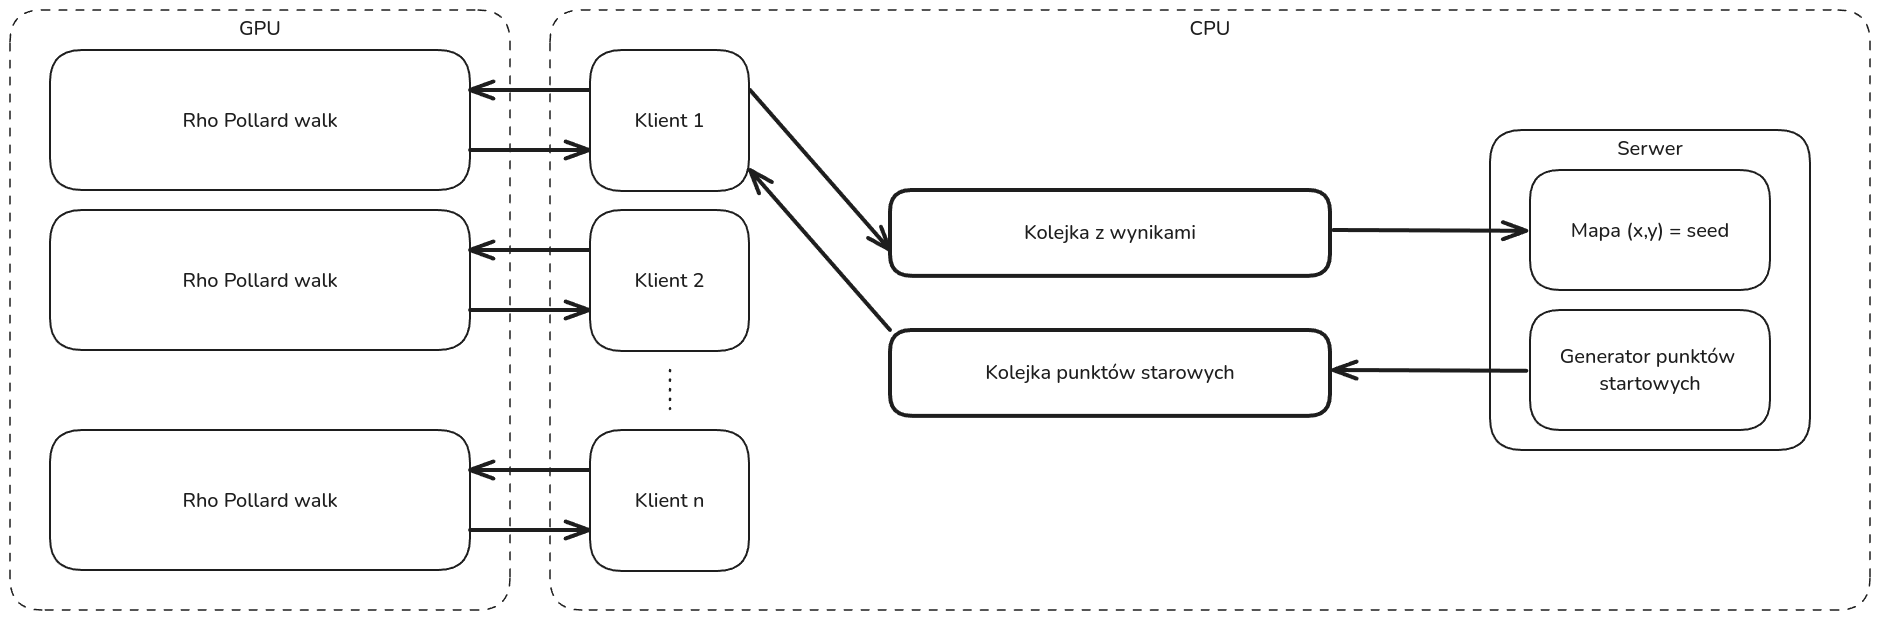
\includegraphics[width=1.1\linewidth]{arch.png}
    \caption{Schemat architektury}
\end{figure}
